\section*{Результаты измерений}

\subsection*{Исследование дифракции Френеля}

С помощью микрометрического винта была установлена ширина щели $0,30 \mm$. С помощью нескольких измерений микроскопом было установлено, что ширина щели равна $0,24 \mm$. Данное расхождение скорее всего связано с тем, что у щели не идеально ровные края. Неровность краев щели была видна, когда полностью закрытую щель освещали лампой, и она всё равно пропускала малую часть света. Поэтому из-за не совсем точного определения момента открытия щели и неровных краев результаты измерений ширины щели отличаются. Далее при расчетах будет использоваться ширина щели, измеренная микроскопом.

\begin{figure}[h]
	\begin{minipage}[h]{0.49 \linewidth}
		\centering
		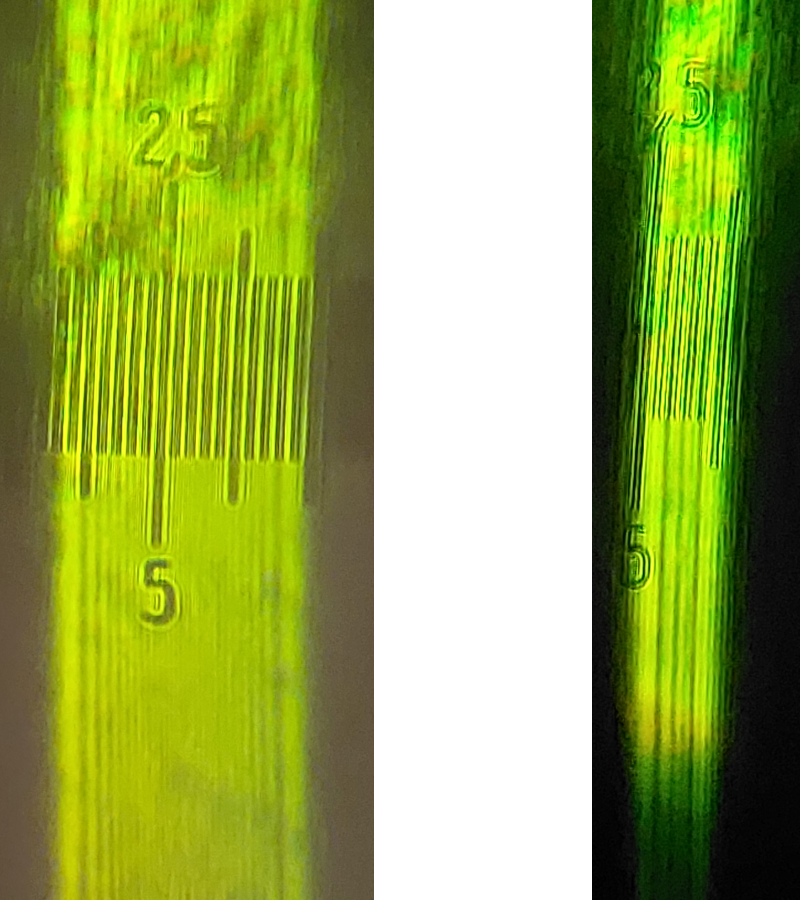
\includegraphics[width=0.8\linewidth]{../Изображения/Качественно Френель размер щели.png}
		\caption{}
		\label{img:Fresnel-diffraction-quality}
	\end{minipage}
	\hfill
	\begin{minipage}[h]{0.49 \linewidth}
		\centering
		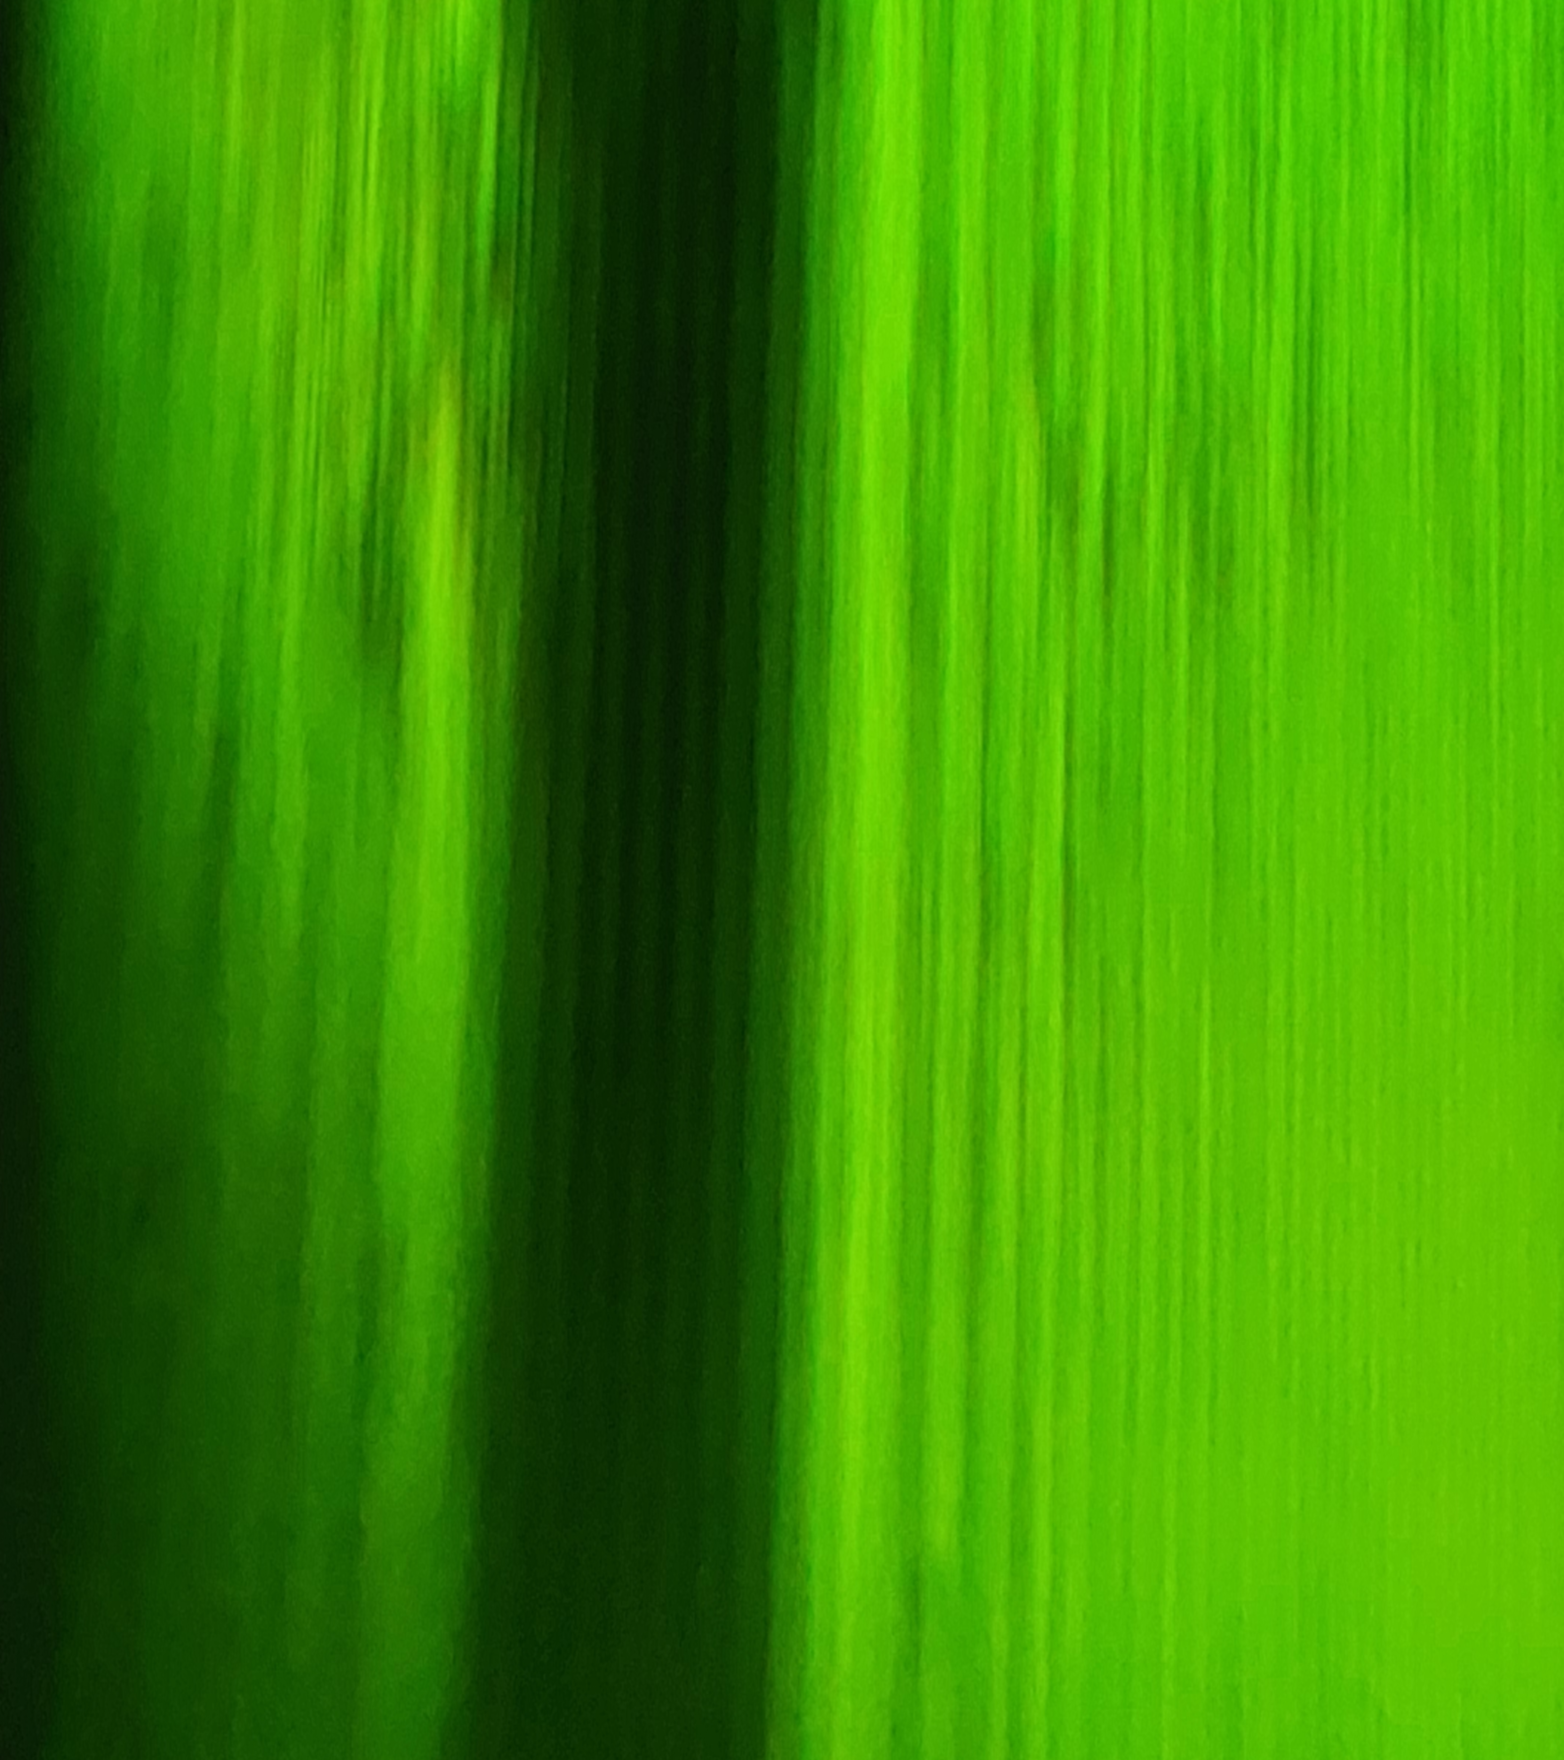
\includegraphics[width=0.8\linewidth]{../Изображения/Пятно Пуассона2.png}
		\caption{}
		\label{img:Poisson-spot}
	\end{minipage}
	\begin{tabular}{p{0.49\linewidth}p{0.49\linewidth}}
		Качественная зависимость дифракционной картины от ширины щели. Слева щель открыта больше, чем справа. Количество черных дифракционных слева больше, чем справа. &
		\centering
		Пятно Пуассона. \\
	\end{tabular}
\end{figure}


В ходе наблюдений было установлено (рис. $\ref{img:Fresnel-diffraction-quality}$), что при неизменном расстоянии до микроскопа, при увеличении размера щели, количество чёрных дифракционных полос увеличивается, они становятся более размытыми и меньше по толщине.

В работе наблюдалась дифракция Френеля на препятствии (рис. $\ref{img:Poisson-spot}$). Из-за большого размера входной щели не удалось количество дифракционных полос большое, при уменьшении размера входной щели, уменьшается яркость картинки. Поэтому точное число тёмных дифракционных полос на фоне нити установить не удалось.

